\subsection{GUI}
\label{GUI}
I dette afsnit vil vi beskrive vores valg i forhold til GUI, hvorfor det ser ud som det gør, og hvad vores PO syntes om det.

\subsubsection{Hvorfor ser vores GUI ud som det gør?}
Det gør det fordi vores PO gerne vil have noget, der er nemt at overskue, og der giver dem den bedste overgang fra deres tidligere system.

Måden vi har gjort det på er ved, at vi har fået adgang til deres nuværende system og har taget en stor inspiration fra deres GUI og kommet vores eget spin på det.

Under møder med PO har de altid lagt meget vægt på brugervenlighed, derfor har vi også forsøgt at holde vores brugergrænseflade så ren som muligt, og derved så overskuelig som muligt, se figur \ref{GUI:Screenshot}.

\begin{figure}[H]
    \caption{Kalendervinduet for Semplito}
    \centering
        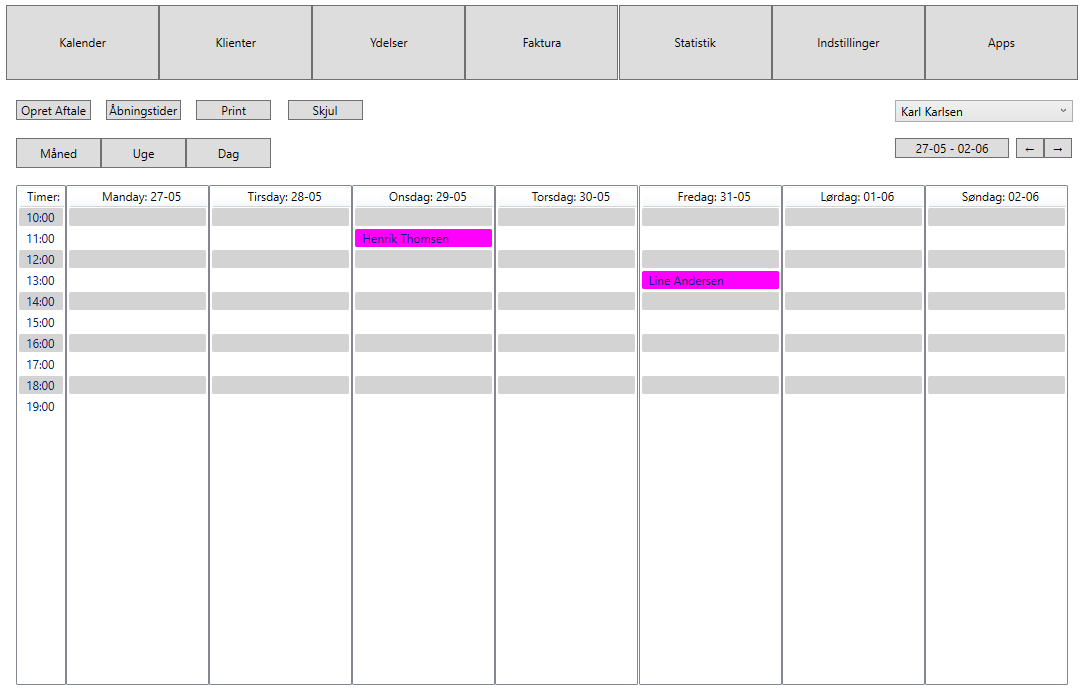
\includegraphics[width=\textwidth]{landingPage.png}
    \label{GUI:Screenshot}
\end{figure}

Vi har valgt at holde det i hvid og grå, da vi ikke har evnerne til at sammensætte farver, så det ser ordentligt ud inden for en begrænset tidsramme, og vi er blevet enige med PO om, at det er en vigtigere prioritering af vores tid at fokusere på funktionaliteten af systemet i stedet for det æstetiske.

\subsubsection{PO's mening:}
Vores PO har hele vejen igennem projektet været meget positiv over, hvad vi har nået, og de har specielt været meget positive i forhold til, hvordan vi har lavet vores wireframe, og hvordan vores GUI er endt op med at se ud.